\documentclass{article}
\usepackage{tikz}
\usetikzlibrary{calc} % ← これを忘れるとエラーになります


%Tikzコマンド-------------------------------------------------
%nodeを二つ渡して、中点に同じ長さの記号(垂直二重線)を書く
%一番目の引数が色で、デフォルトでは赤
\newcommand{\eqlend}[3][red]{
    % 線分を描画
  \draw[thick] (#2) -- (#3);
  
  % 赤く太い、垂直な二重線
    \draw[#1,thick] let
    \p1 = ($ (#3) - (#2) $),
    \n1 = {veclen(\x1,\y1)}, %ベクトルの長さ
    \p2 = ($ (#2) + 0.5*(\p1) $), %中点Mの座標
    \p3 = ($ (#2) + 0.53*(\p1) $), %Mをずらした点N
    \p4 = (0.04*\y1 , -0.04*\x1) %法線方向のベクトル、長さ調整済み
  in {
    ($ (\p2) + (\p4) $) -- ($ (\p2) - (\p4) $) %Mを通る短い垂線
    ($ (\p3) + (\p4) $) -- ($ (\p3) - (\p4) $) %Nを通る短い垂線
  };
}

%nodeを二つ渡して、中点に丸を書く
%一番目の引数が色で、デフォルトでは赤
\newcommand{\eqcircle}[3][red]{
    % 線分を描画
  \draw[thick] (#2) -- (#3);
  
    \draw[#1,thick] let
    \p1 = ($ (#3) - (#2) $),
    \n1 = {veclen(\x1,\y1)}, %ベクトルの長さ
    \p2 = ($ (#2) + 0.5*(\p1) $), %中点Mの座標
    \n2 = {0.03*\n1} %円の半径
  in {
    (\p2) circle (\n2) %Mを通る短い垂線
  };
}

%単位法線ベクトルを出力する
% 引数 #1: 入力ベクトルの始点、#2: 入力ベクトルの終点、#3: 結果を格納
\newcommand{\unitnormal}[3]{
\path let
  \p1 = ($(#2)-(#1)$), %ベクトルAB
  \n1 = {veclen(\x1,\y1)}
  in
  coordinate (#3) at (-\y1/\n1 , \x1/\n1); %単位法線ベクトル
}
%----------------------------------------------------------

\begin{document}

\begin{tikzpicture}
  \node (P1) at (1,1) {P};
  \node (P2) at (5,3) {Q};
  \eqlend[blue]{P1}{P2}
\end{tikzpicture}

\begin{tikzpicture}
  \node (P1) at (1,1) {P};
  \node (P2) at (5,3) {Q};
  \eqcircle{P1}{P2}
\end{tikzpicture}


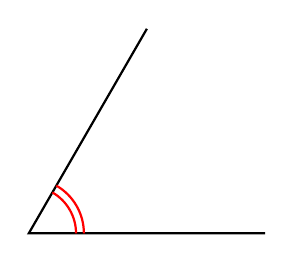
\begin{tikzpicture}
  % 角度60度、半径3の角
  \draw[thick] (60:3) -- (0,0) -- (3,0); 
    %arc[start angle=0, end angle=60, radius=3cm] 
    %-- cycle;

  % 内側の円弧(0度〜60度、半径0.6cm)
  \draw[thick, red] (0.6,0) arc[start angle=0, end angle=60, radius=0.6cm];
  % さらに外側の円弧
  \draw[thick, red] (0.7,0) arc[start angle=0, end angle=60, radius=0.7cm];
\end{tikzpicture}

\bigskip

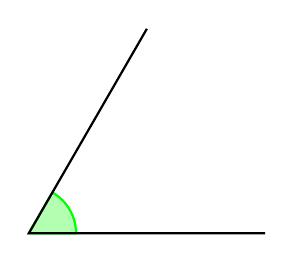
\begin{tikzpicture}
  % 内側の円弧(0度〜60度、半径0.6cm)
  \draw[thick, green, fill=green!30!white] (0,0) -- (0.6,0) arc[start angle=0, end angle=60, radius=0.6cm] --cycle;
  
  % 角度60度、半径3の角
  \draw[thick] (60:3) -- (0,0) -- (3,0); 
\end{tikzpicture}

\bigskip

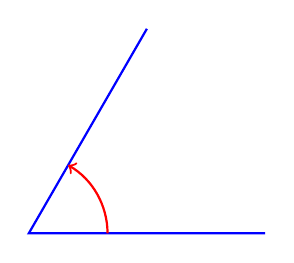
\begin{tikzpicture}

  % 座標AとBの定義
  \coordinate (A) at (3, 0);
  \coordinate (B) at (60:3); % 例: 60度の方向
  \coordinate (S) at (1,0);

  % AとBの角度を計算(度)
  \pgfmathsetmacro{\angleA}{atan2(0,1)}  % atan2(y, x) for A
  \pgfmathsetmacro{\angleB}{atan2(sin(60), cos(60))}  % for B

  % ベクトル
  \draw[thick, blue] (B) -- (0,0) -- (A);
  %\draw[->, thick, blue] (0,0) -- (B) node[above right] {$\vec{b}$};

  % 原点中心の円弧(赤)を描画
  \draw[thick, red, ->] (S) arc[start angle=\angleA, end angle=\angleB, radius=1cm];

  % 点の表示
  %\fill (A) circle (1pt) node[below right] {A};
\end{tikzpicture}

\bigskip

\begin{tikzpicture}
\coordinate (A) at (1,1);
\coordinate (B) at (5,3);
\coordinate (M) at ($(A)!0.5!(B)$); %ABの中点M
\coordinate (N1) at (0,0); %法線ベクトル用の座標を用意

\draw[thick] (A) -- (B);

%線分ABの単位法線ベクトルをN1に出力
\unitnormal{A}{B}{N1}

%Mを通る垂線
\draw[thick, blue] (M) -- ($(M)+60*(N1)$);

%直角記号
\draw ($(M)+10*(N1)$) -- ($(A)!0.57!(B) + 10*(N1)$) -- ($(A)!0.57!(B)$);
\end{tikzpicture}
\end{document}


%https://amusant.hatenablog.jp/entry/2024/09/12/200206
%pip install -r requirements.txt 
%py kemono-dl.py --cookies "cookies.txt" --links https://kemono.su/特定ウェブサイト名/user/ユーザーID
%py kemono-dl.py --links https://kemono.su/patreon/user/9641995